% Choix de l'outil de mise en ligne

Nous avons mentionné deux formes que peuvent prendre les éditions numériques~: un \textit{ebook} ou un site web. Selon la méthode de publication choisie, des connaissances en programmation et en développement web peuvent s'avérer nécessaires. Nous en verrons trois~: la création d'un site à partir des fichiers XML grâce à une transformation XSLT, la création d'une application web, et l'utilisation d'une plateforme de publication.    


\section{Méthodes de publication}

\subsection{Transformation XSLT vers HTML}
XSLT est le langage de transformation de l'environnement XML. Un fichier XSL est une feuille de style qui contient des \enquote{\textit{templates\footcite[chapitre 8]{HaroldMeans2002}}}. Cette feuille de style permet de transformer un fichier XML. Le fichier de sortie peut être un autre fichier XML ou dans un autre format~; dans notre cas, il s'agirait d'un fichier HTML.  

Pour opérer une transformation, il faut indiquer au processeur XSL la position de l'élément à transformer grâce à une expression XPath. Pour chaque type de page web que nous souhaitons créer, il faudra créer un \textit{template} contenant les règles de transformation. Par exemple, dans le cas des éditions EHRI, il faudrait créer des \textit{templates} pour la page d'accueil générale des éditions, pour les collection, et pour l'affichage du document. L'élément \texttt{<xsl:template>} contient donc le code HTML que l'on souhaite voir apparaître dans le fichier de sortie, où chaque élément qui dépend du fichier d'entrée (son titre, par exemple) est identifié par son expression XPath. Cela permet de contrôler le niveau de l'arbre XML où sont appliquées les transformations\footcite[chapitre 8]{HaroldMeans2002}.


\subsection{Création d'une application web}
La création d'une application web requiert des connaissances en programmation. Plusieurs langages sont disponibles pour le développement d'une application web~: Python, JavaScript, PHP, Ruby, etc. Nous nous concentrerons sur le langage Python.  

Comme de nombreux langages de programmation, Python dispose de \textit{frameworks}. Un \textit{framework} permet de développer une application grâce à des outils intégrés. Par exemple, le \textit{framework} Flask \footnote{Documentation de Flask (version 2.3)~: \texttt{\href{https://flask.palletsproject.com/en/2.3.x/}{https://flask.palletsprojects.com/en/2.3.x/}}.} permet de créer des \enquote{routes} (URL) qui afficheront la page web associée au \textit{template} HTML. Cette méthode suppose la création d'une base de données dans laquelle Flask ira chercher les informations pour créer l'affichage du site, ce qui nécessite des compétences supplémentaires en gestion de bases de données.


\subsection{Utilisation d'une plateforme de publication}
Enfin, la troisième méthode, qui est sûrement la plus populaire, est le recours à un système de gestion de contenu (CMS). Cette méthode consiste en l'utilisation d'outils permettant aux chercheur$\cdot$euse$\cdot$s de publier leur édition numérique sans devenir développeur$\cdot$euse$\cdot$s. Nous n'évoquerons dans ce mémoire que deux solutions~: Omeka et TEI Publisher.   



\section{Les éditions EHRI et le logiciel Omeka}
Pour la publication de leurs éditions en ligne, l'EHRI a opté en 2018 pour l'utilisation du logiciel \textit{open source} Omeka\footnote{Omeka~: \texttt{\href{https://omeka.org/}{https://omeka.org/}}.}. C'est un CMS, \enquote{dédié à l'organisation, à l'exposition, à la mise en ligne de données iconographiques, avec leur métadonnées, qui permet d'en faire très facilement une publication sur le Web\footcite[p.~81]{BoulaireCarabelli2017}}. Il est également précisé qu'Omeka est \enquote{spécialisé dans l'édition de collections muséales, de bibliothèques numériques et d'éditions savantes en ligne\footcite[p.~115]{IdmhandRiffardWalter2017}.} Il existe deux versions disponibles d'Omeka avec des fonctionnalités différentes~: \enquote{Omeka Classic}, que nous aborderons dans ce mémoire, et \enquote{Omeka S}, davantage orienté vers le web sémantique\footnote{Pour en savoir plus sur Omeka~: \texttt{\href{https://omeka.org/about/project/}{https://omeka.org/about/project/}}.}.

\subsection{Fonctionnement d'Omeka Classic}
Omeka permet la gestion, la valorisation et la diffusion d'importantes collections numérisées\footcite[p.1]{Leblanc2020}. C'est un outil pensé pour la réalisation d'édition \enquote{numérisées\footcite[p.~27]{Sahle2016}} (\enquote{\textit{digitized edition}}) et non numériques (\enquote{\textit{digital edition}})\footcite[p.~2]{Leblanc2020}.  

Deux utilisations se distinguent de l'utilisation d'Omeka. Le logiciel permet de \enquote{représenter de manière structurée et normalisée des connaissances sur des documents\footcite[diapo 7]{Daussin2019}}, mais également de \enquote{construire des parcours raisonnés à l’aide de pages web dans une sélection ou une collection de
documents\footcite[diapo 7]{Daussin2019}}, et ce à des fins de partage ou de conservation.  

Un \enquote{contenu Omeka\footcite[diapo 8]{Daussin2019}} est composé d'un document et de ses métadonnées~; le document lui-même pouvant être composé de plusieurs fichiers. Les métadonnées sont signalées à l'aide du standard Dublin Core et décrivent le contenu (titre, sujet, description, source,  langue, relation et couverture), la propriété intellectuelle (créateur, contributeur, éditeur et gestion des droits) et l'instanciation (date, type, format, identifiant de la ressource)\footnote{Pour plus d'informations sur le standard Dublin Core~: \texttt{\href{https://www.bnf.fr/fr/dublin-core}{https://www.bnf.fr/fr/dublin-core}} (visité le 02/09/2023).}.


\subsection{Limites posées par le recours à Omeka}
Pour les chercheur$\cdot$euse$\cdot$s souhaitant publier proprement leur édition sans avoir à apprendre la programmation, l'utilisation d'Omeka présente de nombreux avantages. Le logiciel permet notamment de gérer un volume conséquent de données et de valoriser son contenu par la création d'\enquote{expositions virtuelles, \textins{de} cartes et \textins{de} frises chronologiques\footcite[p.~18-19]{Leblanc2020}}.  

Pourtant, et spécifiquement pour la création d'éditions numériques, Omeka présente un inconvénient non négligeable~: le logiciel n'est pas conçu pour traiter des documents encodés en TEI. Ce sont les équipes des projets travaillant sur Omeka qui ont développé des modules (\textit{plug-ins}) pour permettre le traitement et l'affichage de ces éditions\footcite[p.~4]{Leblanc2020}, alors que le standard TEI est le plus utilisé par l'édition scientifique numérique.  

\bigskip
\bigskip
\bigskip
\bigskip
À titre d'exemple, l'équipe éditoriale du WP12 de l'EHRI a dû mettre au point une correspondance entre certains éléments du \texttt{<teiHeader>} et les champs du Dublin Core\footcite[p.~7-9]{Ehri2018} pour pouvoir travailler avec Omeka\footcite[p.~9]{Leblanc2020}. Cette opération s'apparente donc à une sorte de \enquote{bricolage numérique\footcite[p.~96]{BoulaireCarabelli2017}} et nécessiterait systématiquement la présence d'un$\cdot$e ingénieur$\cdot$e dans l'équipe du projet, ce qui est loin d'être le cas en Sciences Humaines et Sociales\footcite[p.~98]{BoulaireCarabelli2017}.  

Enfin, les modules développés par les équipe de projets pour ajouter des fonctionnalités à Omeka en fonction de leurs besoins peuvent ne plus être compatibles avec le logiciel au fur et à mesure de ses mises à jour. En plus du lourd travail de développement nécessaire à la création d'un module, celui-ci doit être maintenu et la compatibilité avec la version courante d'Omeka doit être assurée\footcite[p.~16]{Leblanc2020}. Or, ce sont des missions que les chercheur$\cdot$euse$\cdot$s ne peuvent pas assurer eux$\cdot$elles-mêmes, d'une part parce que c'est une activité très chronophage, et d'autre part parce que cela relève d'un domaine qui n'est pas le leur.  



\section{Une autre alternative~: TEI Publisher}

\subsection{Fonctionnement de TEI Publisher}
TEI Publisher se présente comme un outil permettant aux chercheur$\cdot$euse$\cdot$s et aux éditeur$\cdot$ice$\cdot$s de publier leurs éditions numériques sans apprendre la programmation, tout en laissant une place importante à la personnalisation. Son objectif est de fournir à ses utilisateur$\cdot$ice$\cdot$s une structure fonctionnelle, bien pensée et personnalisable\footnote{Documentation TEI Publisher~: \texttt{\href{https://teipublisher.com/exist/apps/tei-publisher/doc/documentation.xml?odd=docbook&view=div}{https://teipublisher.com/exist/apps/tei-publisher/doc/ documentation.xml?odd=docbook\&view=div}} (visité le 02/09/2023).}.  

Une fois installée, la plateforme est dotée d'une \enquote{aire de jeu\footnote{Disponible depuis la page d'accueil de la plateforme~: \texttt{\href{https://teipublisher.com/exist/apps/tei-publisher/index.html?query=&collection=playground&sort=title&field=text&start=1}{https://teipublisher.com/exist/apps/ tei-publisher/index.html?query=\&collection=playground\&sort=title\&field=text\&start=1}}.}} pour comprendre le fonctionnement de l'outil. L'affichage du document dépend des réglages de l'ODD\footnote{À ne pas confondre avec la documentation de l'encodage du projet d'édition. L'ODD de TEI Publisher permet de gérer l'affichage du document.} choisie. TEI Publisher prend en charge toutes sortes de documents en entrée, et pas seulement des documents encodés en TEI\footcite{Chiffoleau2020}{}, bien qu'il s'agisse du standard recommandé.  

\bigskip
La personnalisation de son application s'effectue à l'aide de modules appelés \enquote{\textit{web components\footnote{Documentation sur les modules~: \texttt{\href{https://cdn.tei-publisher.com/@2.12.6/dist/api.html}{https://cdn.tei-publisher.com/@2.12.6/dist/api.html}}.}}}.


\subsection{Pourquoi choisir TEI Publisher}
TEI Publisher est un outil \textit{open source} et bien documenté. Sa communauté est très active et la plateforme est mise à jour régulièrement\footnote{La dernière version de TEI Publisher (8.0) a été publiée le 28 mars 2023~: \texttt{\href{https://www.e-editiones.org/posts/tei-publisher-8/}{https://www.e-editiones.org/posts/tei-publisher-8/}}.}. De nombreux projets d'éditions numériques utilisent désormais TEI Publisher, et les nouvelles fonctionnalités développées pour un projet en particulier sont mises à disposition des autres utilisateur$\cdot$ice$\cdot$s. C'est un avantage non négligeable par rapport au logiciel Omeka.  

La capacité de l'outil à prendre en charge des formats comme le DOCX\footnote{Format du traitement de texte Microsoft Word.} est un avantage pour les utilisateur$\cdot$ice$\cdot$s qui n'auraient que peu, voie aucunes, compétences en encodage TEI. À titre d'exemple, les éditeurs du WP12 de l'EHRI encodent leurs documents à l'aide d'un traitement de texte simple avec des liens hypertextes. Le fichier est ensuite transformé en XML-TEI avec l'outil \enquote{Odette\footnote{Odette~: \texttt{\href{https://obvil.huma-num.fr/odette/}{https://obvil.huma-num.fr/odette/}}.}}. En utilisant TEI Publisher, cette étape deviendrait superflue et le travail s'en trouverait accéléré.  

En outre, il nous semble important de souligner que TEI Publisher propose un affichage horizontal des documents (Figure \ref{fig:doc-teipublisher}). Les éditions en ligne de l'EHRI disposent d'un affichage vertical (Figure \ref{fig:ehri-omeka}) centré sur la transcription. Or, cet affichage ne nous semble pas des plus pratiques, notamment en raison du peu d'importance qui est accordé au fac-similé.  

\begin{figure}[!h]
    \centering
    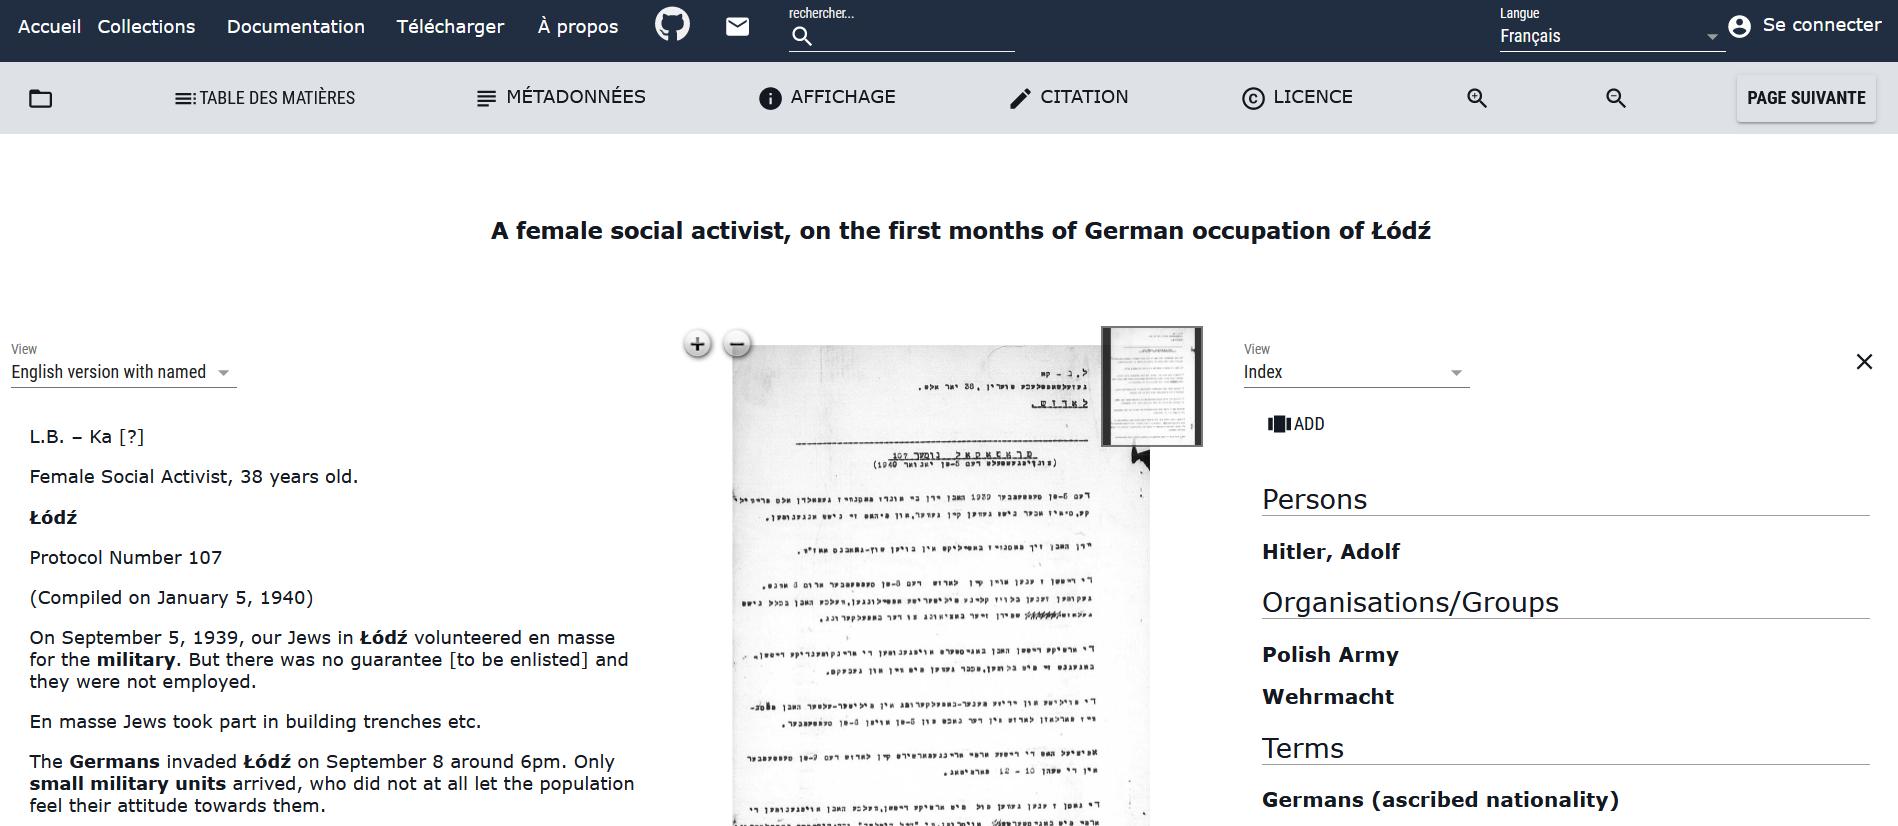
\includegraphics[width=\linewidth]{2-MAIN/images/discholed-document.png}
    \caption{Disposition horizontale avec TEI Publisher (Source~: DiScholEd)}
    \label{fig:doc-teipublisher}
\end{figure}

\begin{figure}[h]
    \centering
    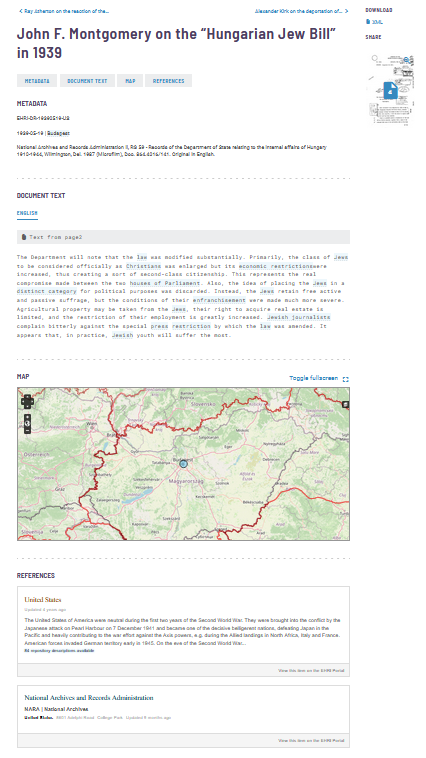
\includegraphics{2-MAIN/images/ehri-omeka.png}
    \caption{Diposition verticale avec Omeka (Source~: EHRI Online Editions)}
    \label{fig:ehri-omeka}
\end{figure}